\section*{Sources of bias in the SQF data}
\begin{figure}
    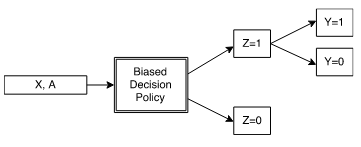
\includegraphics[width=0.7\textwidth]{../figures/selection_bias.png}
    \caption{Selection bias in the SQF data.}
    \label{fig:selection_bias}
\end{figure}
The major concern that has been raised in the literature for SQF data is how the data is generated. In their paper "Residual Unfairness" \cite{kallus2018} conceptualize the problem as shown in \autoref{fig:selection_bias}.
We define a person by their sensitive feature (A) and non-sensitive features (X). For each person in the population of interest a police officer decides whether to stop them or not. This is the first potential source of bias. In the SQF context we can imagine that the police is generally more suspicious towards PoC than white people. Or we can imagine that they are stopping people in general more frequently in high crime areas which happen to be correlated with low-income neighbourhoods which are more populated by PoC than white people {\color{red}sources}. Based on this biased decision policy people are included in the sample (Z = 1) or they are not (Z = 0). But naturally, we can only know the outcome of a stop for the people who were stopped.
\cite{kallus2018} distinguish between target population and training population in such scenarios. The target population is the one on which we want to use the ADM on while the training population are the observations the biased decision policy chose to include in the sample and on which the algorithm is trained.
In the SQF data we can see this form of bias by comparing the race distribution of NYC to the race distribution in the SQF data. From \autoref{fig:race_distributions} it is clear that in terms of race the SQF data does not represent the general population of the city. We can see that white people form the majority of the population in NYC, but only make up a tiny fraction of SQF stops. Black people in contrast are the third-largest ethnic group in NYC while they exceed any other group in the SQF data by far.
\autoref{fig:race_distributions} shows that selection bias might be at play in the decision of stopping a suspect.


We take the borough as the non-sensitive variable that in combination with the race describes the suspect.  The comparison of the race distribution in each borough for the SQF data and the New Yorker population as a whole supports the argument that black people are stopped more leniently \autoref{fig:arrestment_rates_clean_data}. The questions now are, why the group metrics did not detect any unfairness in our algorithm and how such biases can be addressed in fairness practice? \\
% The main message of this paper is that it is not that easy to adjust for fairness, when the data the algorithm learns from is biased. Ensuring Equal Opportunity or Equalized Odds on the training data does not generalize to the target population. The paper proposes a way to estimate the TRP and FPR in the target population. This is useful, when the fairness methods depends on the FPR and/or TPR. 
Why the group metrics did not show any unfairness in the algorithm can be answered ins a straight forward way. Group metrics offer a rather isolated view on fairness. They assess disparities in algorithimic predictions between protected groups rather than measuring the fairness of a whole situation. Thus, group metrics are not designed to detect selection bias. They work with the joint distribution of $Y, A, \hat{Y}$ \footnote{There are variations of group metrics that allow for non-sensitive attributes $X$ to be considered as well when assessing fairness. An example is conditional statistical parity \cite{verma2018}.} 
and do not take any additional information into account. When we rely on the true label $Y$ (Separation) to detect unfairness but the true label itself is not reliabel (not generated via an objective truth), then the group metrics cannot show this mechanism \cite{castelnovo2022}.
To answer the second question we use the following chapter to examine two papers that propose methods to address selection bias in fairness practice and have explicity used the SQF data as a case study.

\begin{figure}
    \centering
    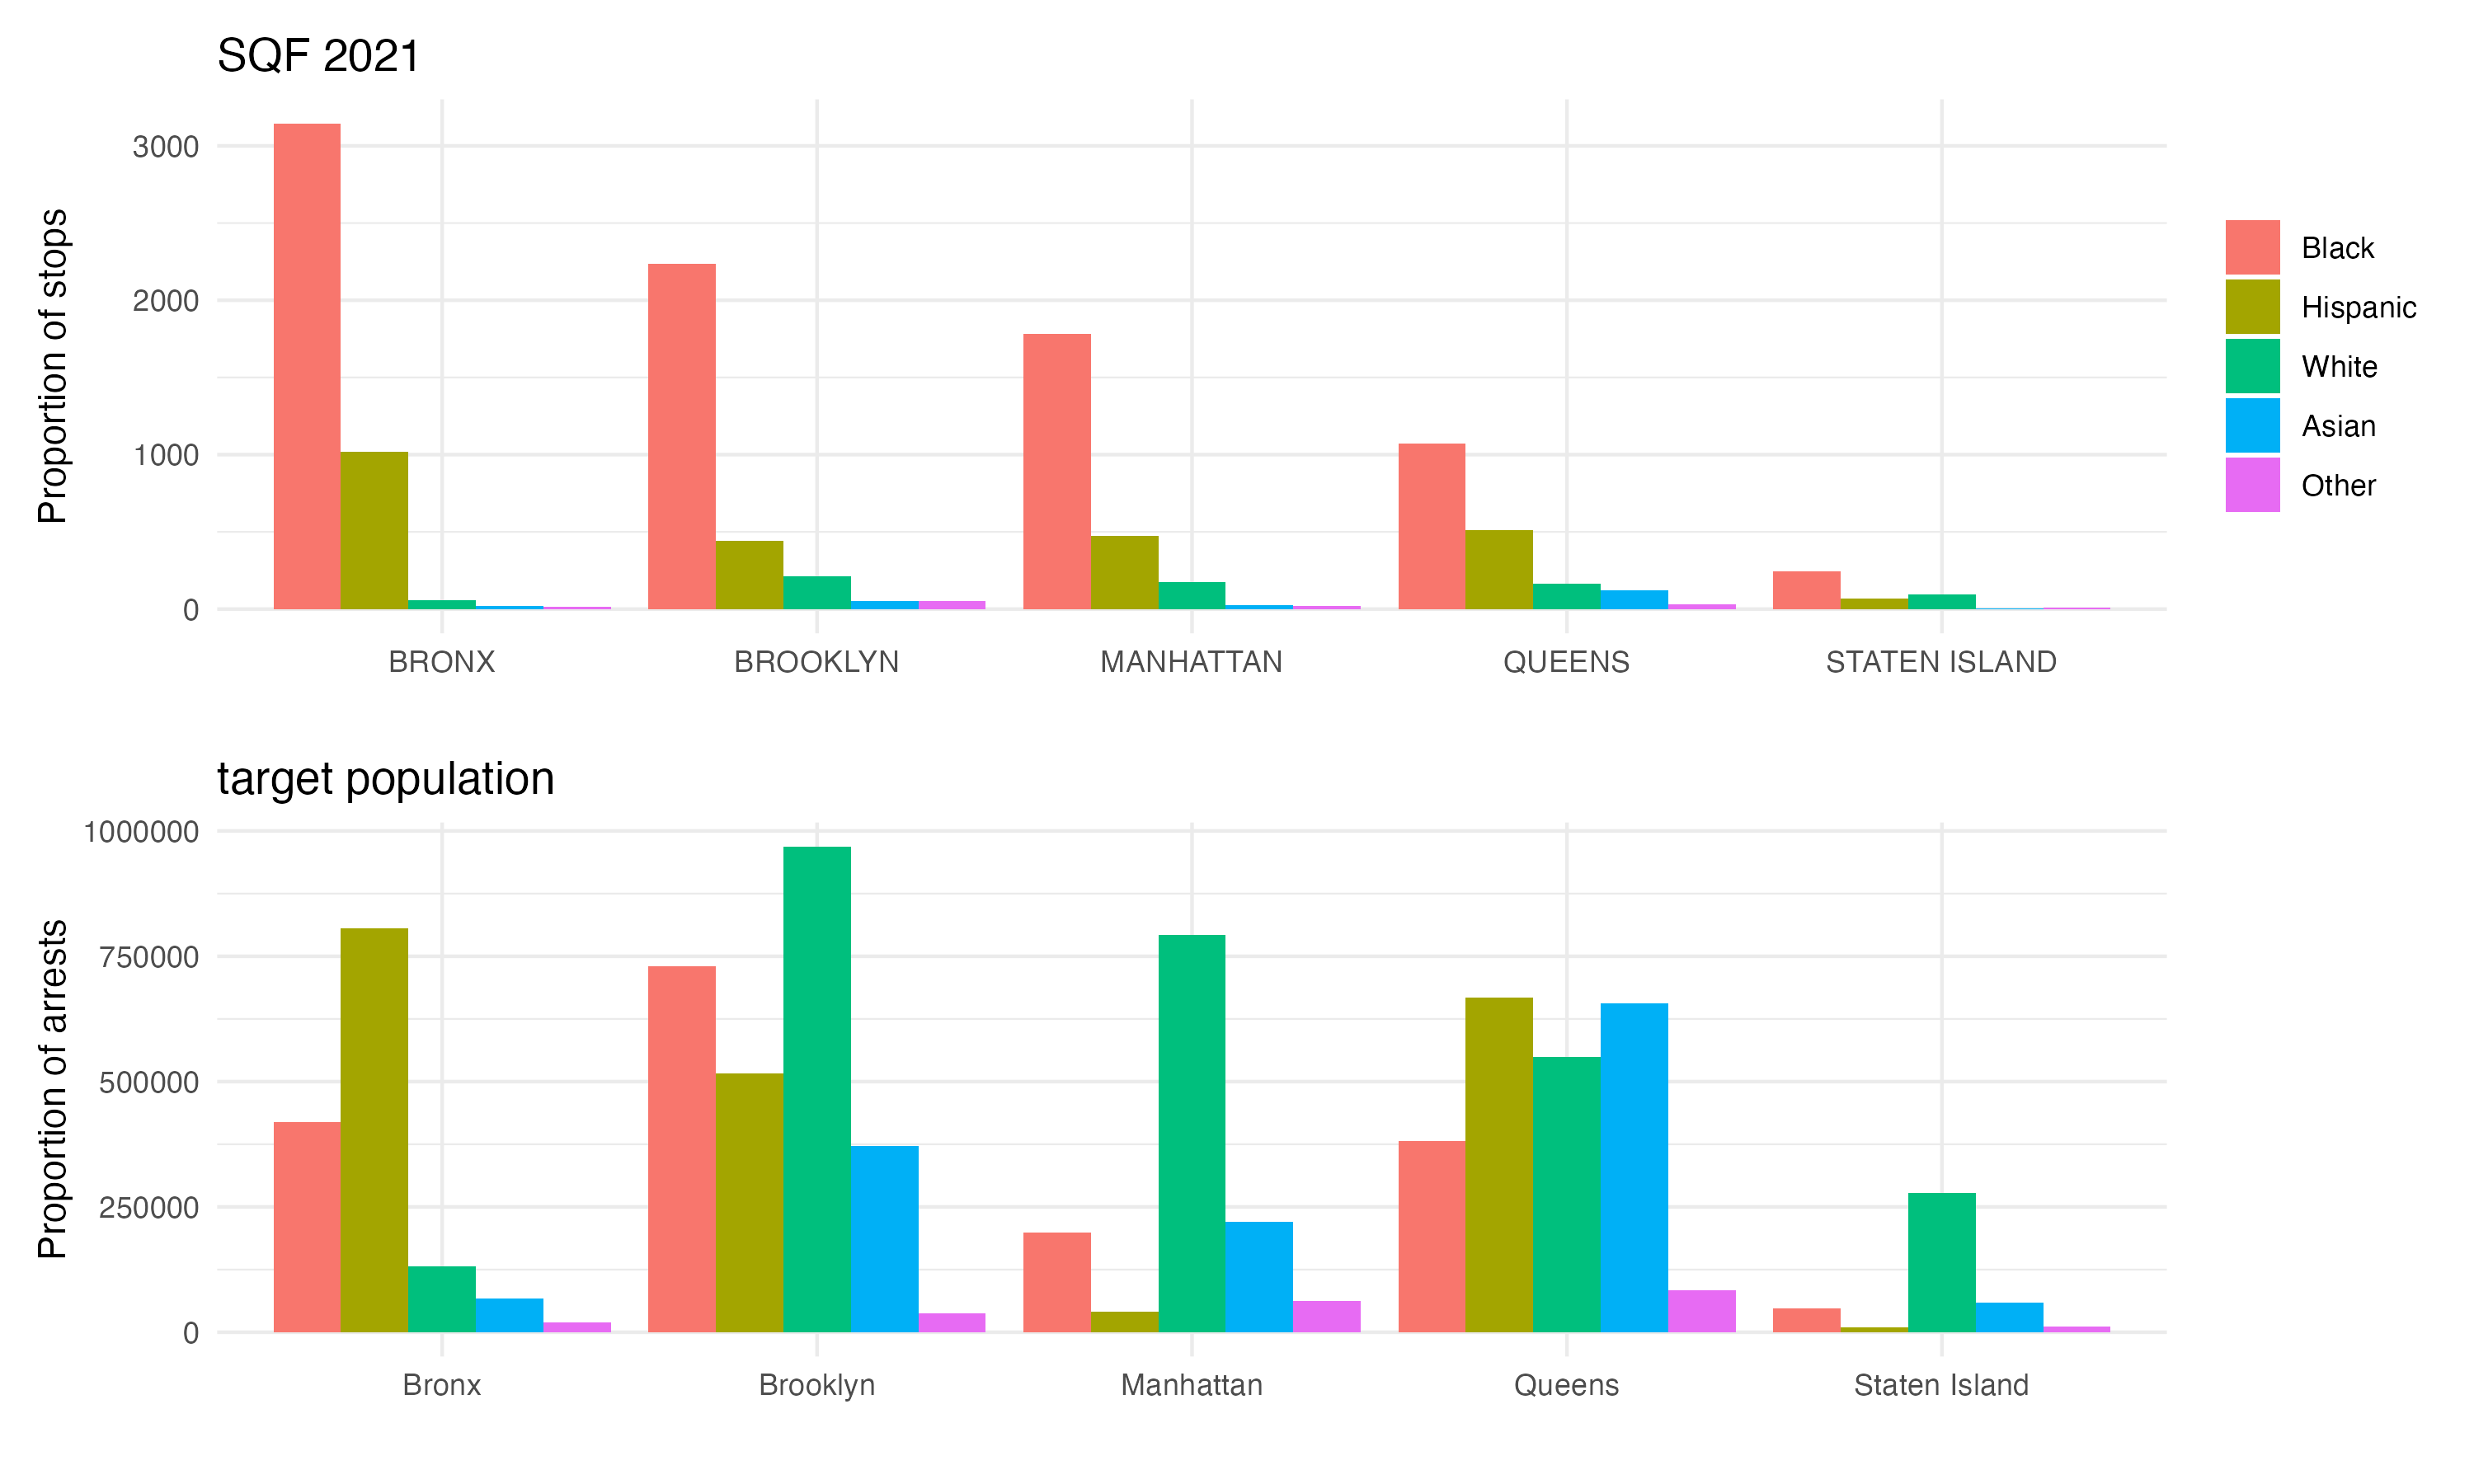
\includegraphics[width=0.7\textwidth]{../figures/sqf_case_study_plot11.png}
    \caption {Distribution of race by borough in the SQF data (top) and NYC as a whole (bottom).}
    \label{fig:borough_race_distribution}
\end{figure}

\section{Residual Unfairness}
We already outlined the formal problem setting in \cite{kallus2018} in \autoref{fig:selection_bias}. The main message of the paper supports the saying "bias in, bias out". They argue that fairness traidional fairness interventions on the training data, such as thresholding, are not enough to ensure fainress in general future applications fo the algorithm. We will take the main findings of the paper and translate them to the SQF scenario.

% Notation and problem setting
Additional notation: $Z$ is the decision of the biased inclusion policy ($Z= 1$ means the subject is included into the training population). $T$ indicated whether a person is in the target population ($T = 1$) means that we want to use the trained algorithm on the person. $\hat{R} \in [0,1]$ is the prediction score.
The problem depicted in \autoref{fig:selection_bias} can be now expressed as follows. We only have knowledge about $X, A, Y | Z = 1$ while we do not know $X, A, Y | Z = 0$. All information about the stop, the demographic details of the person and the outcome which serve as training label for an algorithm are only observed for stopped individuals.

% Fairness definition
The paper defines fairness via equal opportunity. Equal opportunity demands that the true positive rates across groups are equal, so that truly arrested individuals are predicted as such. In our case, in which a positive prediction $\hat{Y} = 1$ is undesirable it makes more sense to look at the false positive rates (or equivilantely at the true negative rates) and define fairness via predictive equality, i.e. $P(\hat{Y} = 1 | Y = 0, A = a) = P(\hat{Y} = 1 | Y = 0, A = b)$ or $P(\hat{Y} = 0 | Y = 0, A = a) = P(\hat{Y} = 0 | Y = 0, A = b)$.
The paper looks at a thresholding classifier, if the prediction score exceeds a certain threshold the positive value for the target is predicted.
This allows us express the false positive rate and the true negative rate of a group $a$ with respect to an event $E$ via the cummulative distibution function. $F_a^E = P(\hat{R} \leq \theta | Y = 1, A = a, E)$. Note that we condition on the truly negative subject in the sample. In the SQF case this would mean that we only look at people that were innocent, so not arrested.
The truly arrested that have a predicted probability $\hat{R} \leq \theta$ are wrongly classified as not-arrested, while the ones for whom $\hat{R} > \theta$ are correctly classified as arrested. $F_a^Z$ gives us nothing other than the false negative rate in the training population and $F_a^T$ is the false negative rate in the target population.
When we want to define a predictive equality classifier on the training population we require $F_a^Z(\theta_a) = F_b^Z(\theta_b)$ to hold. 

% Definition of fair classifier 
An optimal derived predictive equality classifier can then be defined as $\hat{Y} = I(\hat{R} > \theta_A)$ and $F_a^Z(\theta_a) = F_b^Z(\theta_b)$ for all groups a,b. In words, the classifier predicts the positive (undesirable)  outcome with a group-specific threshold for each member of the group while this group specific threshold is set in such a way that predictive equality on the training data is fulfilled. We will not go into detail of how one finds such a classifier but refer to \cite{hardt2016} who propose a post-processing method to derive the optimal thresholds for each group. 

% Definition of unfairness inequity of predictive equality
With the definition of fairness as predictive equality (equal tnr/fpr across groups) we can in turn define unfairness as nothing other than the difference in true negative rates between groups, i.e. \(\epsilon_{a,b}^E = P(\hat{Y} = 0 | Y = 0, A = a, E) - P(\hat{Y} = 0 | Y = 0, A = b, E)\) and call this inequity of predictive equality. $\epsilon_{a,b}^{T=1} > 0$ shows discrimination against group b, since this means that the true negative rate for group b is lower than for group a.
When we construct an equal opportunity classifier (via some fairness intervention) then $\epsilon_{a,b}^{Z=1} = 0$ holds for this classifier. This also means that any unfairness that might show in the target population cannot be explained via existing ineuqities between groups in the training population but via existing differences in the training and the target population. So it is unfairness that gets introduced when we try to generalize our algorithm to the population it was not trained on. \cite{kallus2018} call this residual unfairness, since this is unfairness remaining event after fairness adjustments.

% Scenarios of discrimination
\subsubsection*{Strong disparate benefit of the doubt}
To fully understand the results of the paper, we additionally introduce the concept of stochastic dominance, originating from decision theory. Let $F, G$ be two cummulative distribution functions. Then $G$ first order stochastically dominates $F \preceq G$ when $F(\theta) \geq G(\theta)$ $\forall\theta$. Recall that G and F are cumulative distribution functions. So first order stochastic dominance of G over F, smaller values of G for each input value $\theta$, that the population described by the CDF of G consistently has higher probability values than population F. Their probability mass is concentrated towards the higher input values thus the cummulative distribution function is small for small input values.
Equipped with these definitions the paper constructs difference scenarios of (un)fairness. The bottom line is always that equal opportunity in the training population does not guarantee equal opportunity in the target population. We will introduce the one scenario mathemtically aligning the statements of the paper with the sqf scenario and will only conceptually explain the oterh scenarios which are extensions of the first one.

% Scenario 1: Strong disparat benefit of the doubt (Prop. 2)
We assume the following:
$F_a^{Z=1} \succeq F_a^{T=1} and F_b^{Z=1} \preceq F_b^{T=1}$ and at least one of the equalities does not hold (either $F_a^{Z=1} \ne F_a^{T=1}$ or $F_b^{Z=1} \ne F_b^{T=1}$ or both).
Then every derived equal opportunity classifier has nonnegative inequity of predictive equality for group b relative to group a $\epsilon_{a,b}^{T=1} \geq 0$ and at least one derived equal opportunity classifier will have a strictly positive inequity of predictive equality disadvantaging group b relative to group a $\epsilon_{a,b}^{T=1} > 0$.

In words this means that for group a in the training population we have way more people with high scores (propbabilities of getting positive (undesirable) prediction) than in group a of the target population.
So group a members were stopped very carefully. For group b members the opposite is true. In the train population of group b, there are many more people with low risk scores than there are in the target population of group b. This means group b members were stopped very leniently. 
This aligns with the fact that the sqf data records considerably more stops for black people than white people. In this case the propositions of the paper will show us again that even after adjusting for equal error rates, the classifier will disadvantage group b when applied to the target population.
The results of the paper would then say that adjusting a classifier for predictive equality, so equal false positive rates across groups, is not enough to ensure fairness on a whole and in future application. 

% Extentions of scenario 1
The paper admits that the assumptions are strict and in reality unlikeliky to be met. The assumptions would mean that the police is so biased against group b members that the proportion of low-risk group b members among stopped individuals is higher than the proportion of low-risk gorup b members in the general population. This would require a very unreasonable stopping policy.
Therefore in the propositions that follow they weaken the assumptions. They allow that the stochastic dominance works in the same direction for both groups but the difference in training and target population for group b is so much more different than for group a that discrimination persists.
Recall that the fairness definition of the paper is based on true positive rates and they are especially interested in the post-processing method by Hardt et al. The method takes as input the error rates of a classifier (e.g. the false positive and true positve error rates) in order to find group-specific thresholds that equalise these error rates across groups.
If we now put in the "wrong" error rates, the error rates of the training population, which, however, are nto representative for the target population due to selection bias, we estimate the wrond thresholds. Therefore Kallus and Zhou offer a way to estimate the error rates in the target population based on training data and some additional information.
These "corrected" error rates can then be used to create fairness interventions that will also spill over to the target population. Their approach is interesting and they use it on the SQF data themselves, but it is also very tailored towards error-rate-based group metrics and is mostly useful when the fairness method relies on the error rates, such as the thresholding by Hardt et al. When the fairness methods does not take error rates as an input, there is little use in estimating them for the target population.
Though it could be interesting regardless, to get picture for how the algortihm could generalise.

As the fairness audit in the previous chapter showed little disparities, we only take their method to estiamte the generalisation of the algorithm.
We match the target population to the training population via precinct.
....
Results:
On the target population FPR for POC is estimated to be higher than for white people, but true positive rate also. FNR is estimated lower for POC than for white people on the target population and TNR is estimated to be lower for POC than for white people. So in general POC in the target population are more often expected to be more often predicted as positive and less often as negative. 

For the train population the FPR of black and white people is basically the same whereas the difference in estimated FPR for the target population is a larger (still small) with POC having the higher FPR than white people. High FPR is undesirable.
But at the same time the TPR in the train population is basically the same between groups whereas the for the target population POC get estimated a higher TPR than white people.
So maybe it is better put this way: It is estimated that the classifier performs better in terms of TPR on the POC of the target population than on the white people of the target population. Naturally with a higher TPR comes also a higher FPR (inherent trade-off).
So the estimation overall show minor differences in race groups and at most maybe even a slightly better estimated performance for POC than for white people.



% Things I have to introduce when I want to presente the math of the paper (e.g.Preposition 2)
% - Stochastic dominance
% - derived equal opportunity classifier
% - inequity of opportunity (epsilon)
% - Fairness defintion (equal tnr; predictive equality)